\documentclass[aspectratio=169]{beamer}

\usepackage[croatian]{babel}
\usepackage[T1]{fontenc}
\usepackage[utf8]{inputenc}
\usepackage{lmodern}
\usepackage{microtype}
\usepackage{csquotes}
\usepackage[natbibapa]{apacite}
\usepackage{fontawesome}
\usepackage{listings}

\definecolor{twitterBlue}{HTML}{1DA1F2}

%%%%% titlepage
\title[]{Rad s tabličnim podacima}

\author[]{\fontsize{8}{10}\selectfont Denis Vlašiček\\[.15em]
    Odsjek za psihologiju FFZG | CROSSDA\\[.15em]
    \faEnvelope\ dvlasice@ffzg.hr\\[.15em]
    \textcolor{twitterBlue}{\faTwitter} @dvlasicek\\[.15em]
    \faGithub\ vdeni}

\titlegraphic{\vspace*{-2em}\includegraphics[scale=.30, keepaspectratio=true]%
    {images/walrus-inspector-sheet.pdf}}

\date[]{}
%%%%%

%%%%% prilagodba referenci na hrvatski
\renewcommand{\BCBT}{}
\renewcommand{\BCBL}{}%  comma before last author when no. of authors > 2
\renewcommand{\BOthers}[1]{i sur.\hbox{}}% ``and others''
\renewcommand{\BBAA}{i}
\renewcommand{\BBAB}{i}
\renewcommand{\BIn}{U:}
\renewcommand{\BED}{Ur.\hbox{}}
\renewcommand{\BEDS}{Ur.\hbox{}}
\renewcommand{\BPGS}{str.\hbox{}}
\renewcommand{\BRetrievedFrom}{Preuzeto s:\hbox{}}
\renewcommand{\BEd}{izdanje}
\renewcommand{\BVOL}{svezak}
%%%%%

\setcounter{tocdepth}{1}

%%%%% beamer tema
\usetheme{CambridgeUS}

\usecolortheme{dove}

\setbeamertemplate{itemize items}[default]

\setbeamertemplate{itemize item}{\textbullet}
\setbeamertemplate{itemize subitem}{\(\triangleright\)}

\setbeamertemplate{section page}{
    \begin{centering}
        \Large
        \insertsection\par
    \end{centering}
}

% \setbeamertemplate{footline}{%
%     \hspace*{1em}%%
%     \insertframenumber\,/\,\inserttotalframenumber%
%     \hspace*{\fill}%
%     }

\setbeameroption{hide notes}
%\setbeameroption{show only notes}
%\usepackage{pgfpages}
%\setbeameroption{show notes on second screen=left}

%%%%%

%%%%% serif font kao default
\usefonttheme{serif}
%%%%%

\setbeamertemplate{navigation symbols}{}

\makeatletter
\newenvironment{noheadline}{
    \setbeamertemplate{headline}{}
}{}
\makeatother
%%%%%

%%%%% nastavljanje enumerate
\newcounter{saveenumi}
\newcommand{\seti}{\setcounter{saveenumi}{\value{enumi}}}
\newcommand{\conti}{\setcounter{enumi}{\value{saveenumi}}}

\resetcounteronoverlays{saveenumi}
%%%%%

%%%% fontsize za bibliografiju
\renewcommand*{\bibfont}{\scriptsize}
%%%%%

%%%%% tiny citep
\newcommand{\tinycitep}[1]{%
    \bgroup
    \scriptsize
    \citep{#1}
    \egroup}
%%%%%

%%%% listings
\lstset{basicstyle=\footnotesize\ttfamily}

\begin{document}

\begin{frame}
    \titlepage
\end{frame}

\section{Uvod}

\begin{noheadline}
    \begin{frame}
        \sectionpage
    \end{frame}
\end{noheadline}

\begin{noheadline}
    \begin{frame}
        \frametitle{Uvod}

        \leavevmode

        \makebox(0, 0){%
        \put(10, 50){
\includegraphics[scale=.40]{images/excel-at-covid.png}}}

        \pause

        \makebox(0, 0){%
        \put(90, 0){
\includegraphics[scale=.40]{images/rename-genes.png}}}

    \end{frame}
\end{noheadline}

\section{Kako se obraniti od ružnih podataka?}

\begin{noheadline}
    \begin{frame}
        \sectionpage

        \begin{center}
            
\includegraphics[scale=.35]{images/walrus-combat-sheet.pdf}
        \end{center}
    \end{frame}
\end{noheadline}

\begin{noheadline}
    \begin{frame}
        \frametitle{Kako se obraniti od ružnih podataka?}

        \begin{columns}

            \column{.50\linewidth}

            \begin{itemize}
                \setlength{\itemsep}{2em}

                \item što god radili, budite konzistentni

                \vspace{1em}
                
                \pause

                    \begin{itemize}
                        \setlength{\itemsep}{2em}

                        \item konzistentna imena varijabli

                        \item konzistentne oznake vrijednosti

                        \item konzistentna imena datoteka

                        \item konzistentan format datuma (\texttt{YYYY-MM-DD};
                            npr. \texttt{2020-12-04})

                    \end{itemize}
            \end{itemize}

            \pause

            \column{.50\linewidth}

            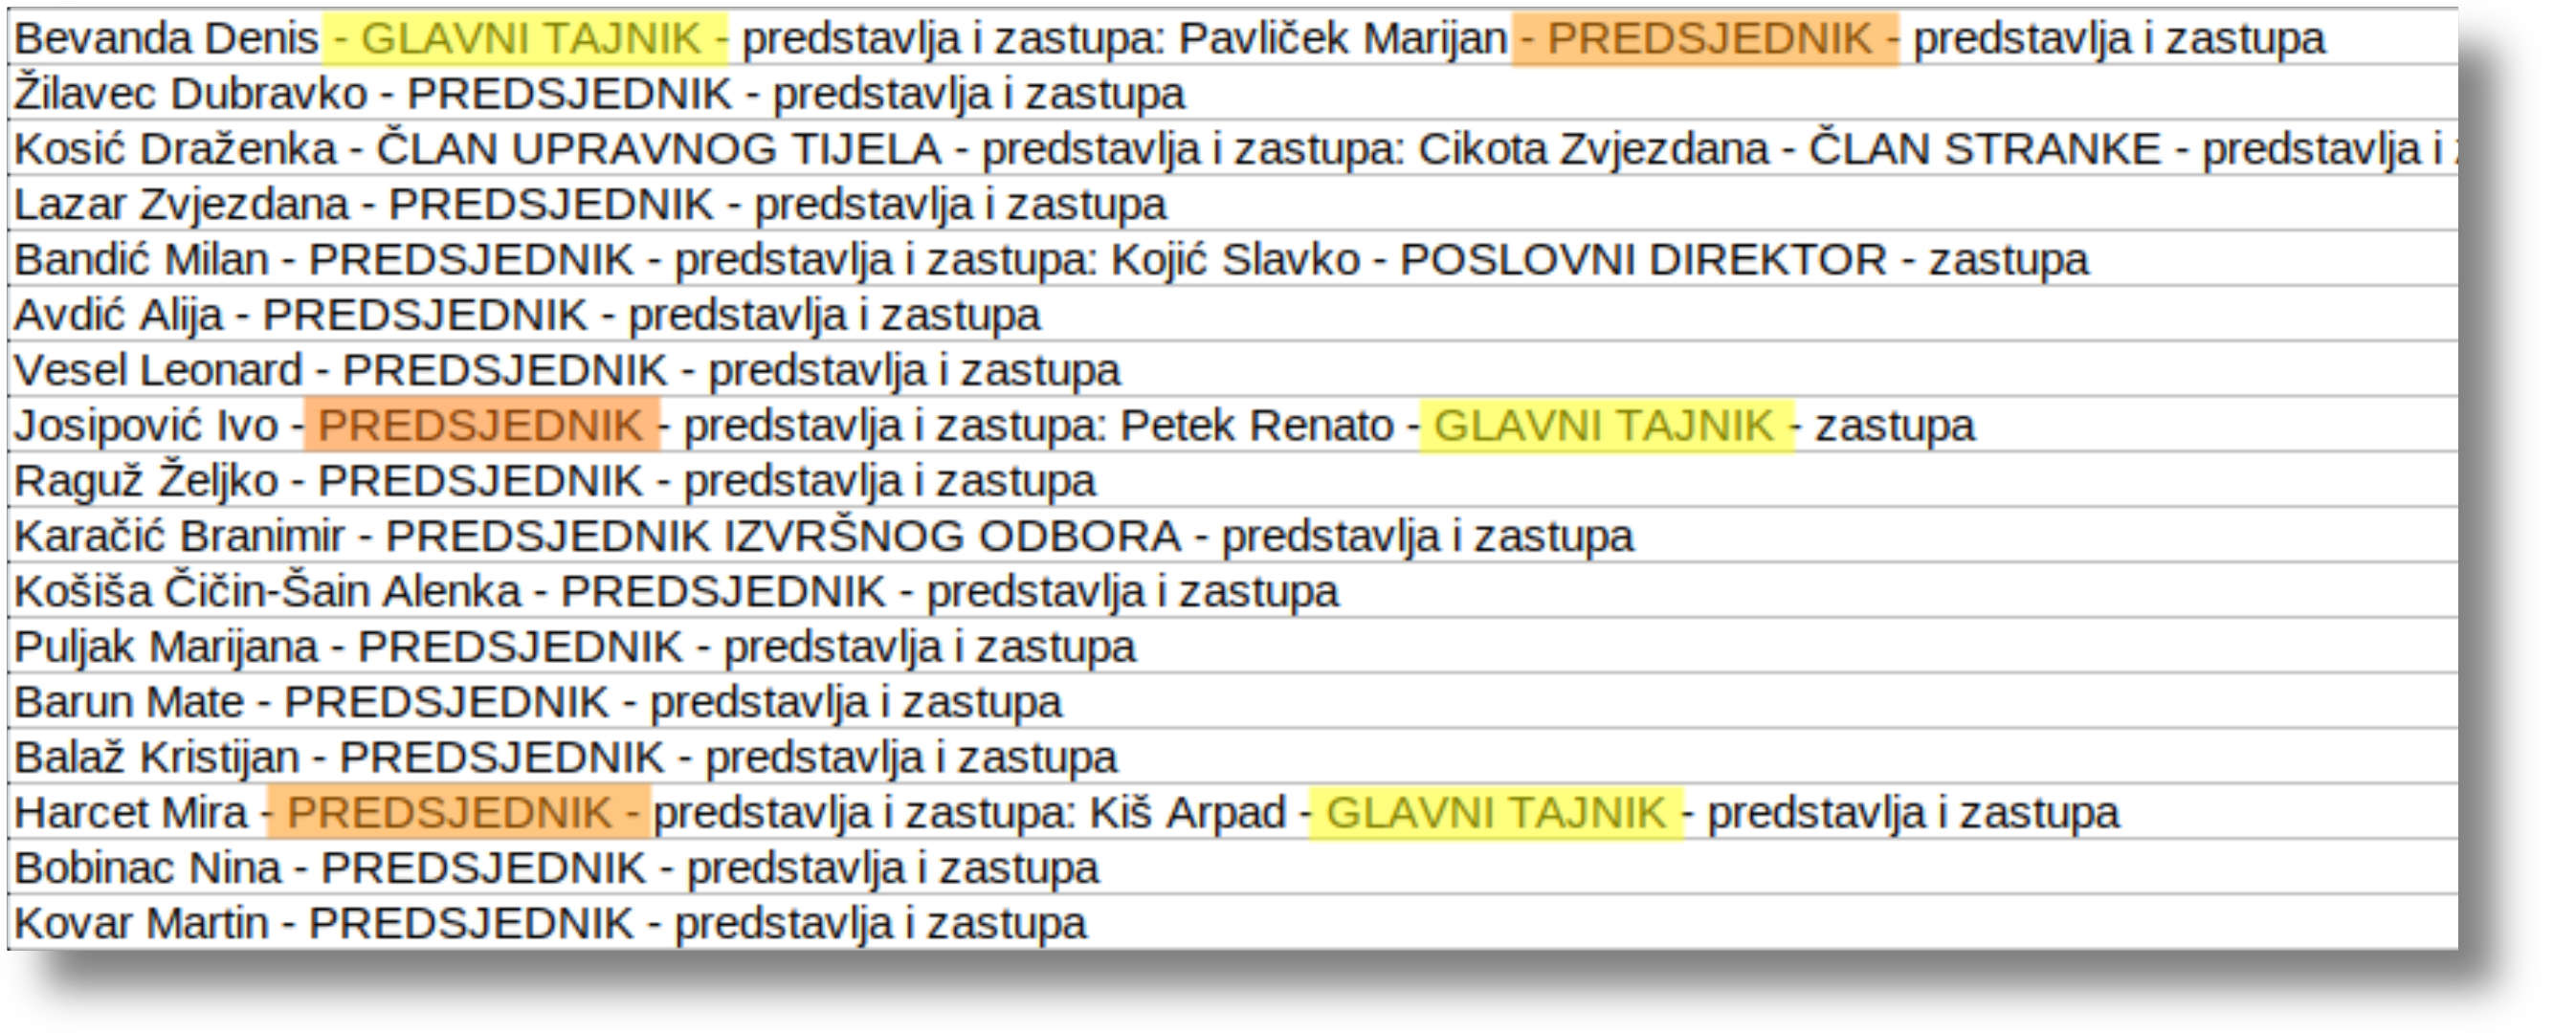
\includegraphics[scale=.30]{images/konzistentan-predsjednik.png}

        \end{columns}
    \end{frame}
\end{noheadline}

\begin{frame}
    \begin{itemize}
        \setlength{\itemsep}{2em}

        \item u \textit{jednu} ćeliju stavite samo \textit{jedan} podatak

        \item ne ostavljajte prazne ćelije

            \begin{itemize}
                \item ako vrijednost \textit{treba} nedostajati, stavite
                    eksplicitnu oznaku (na primjer \texttt{NA})

            \end{itemize}

        \vspace{1.5em}

        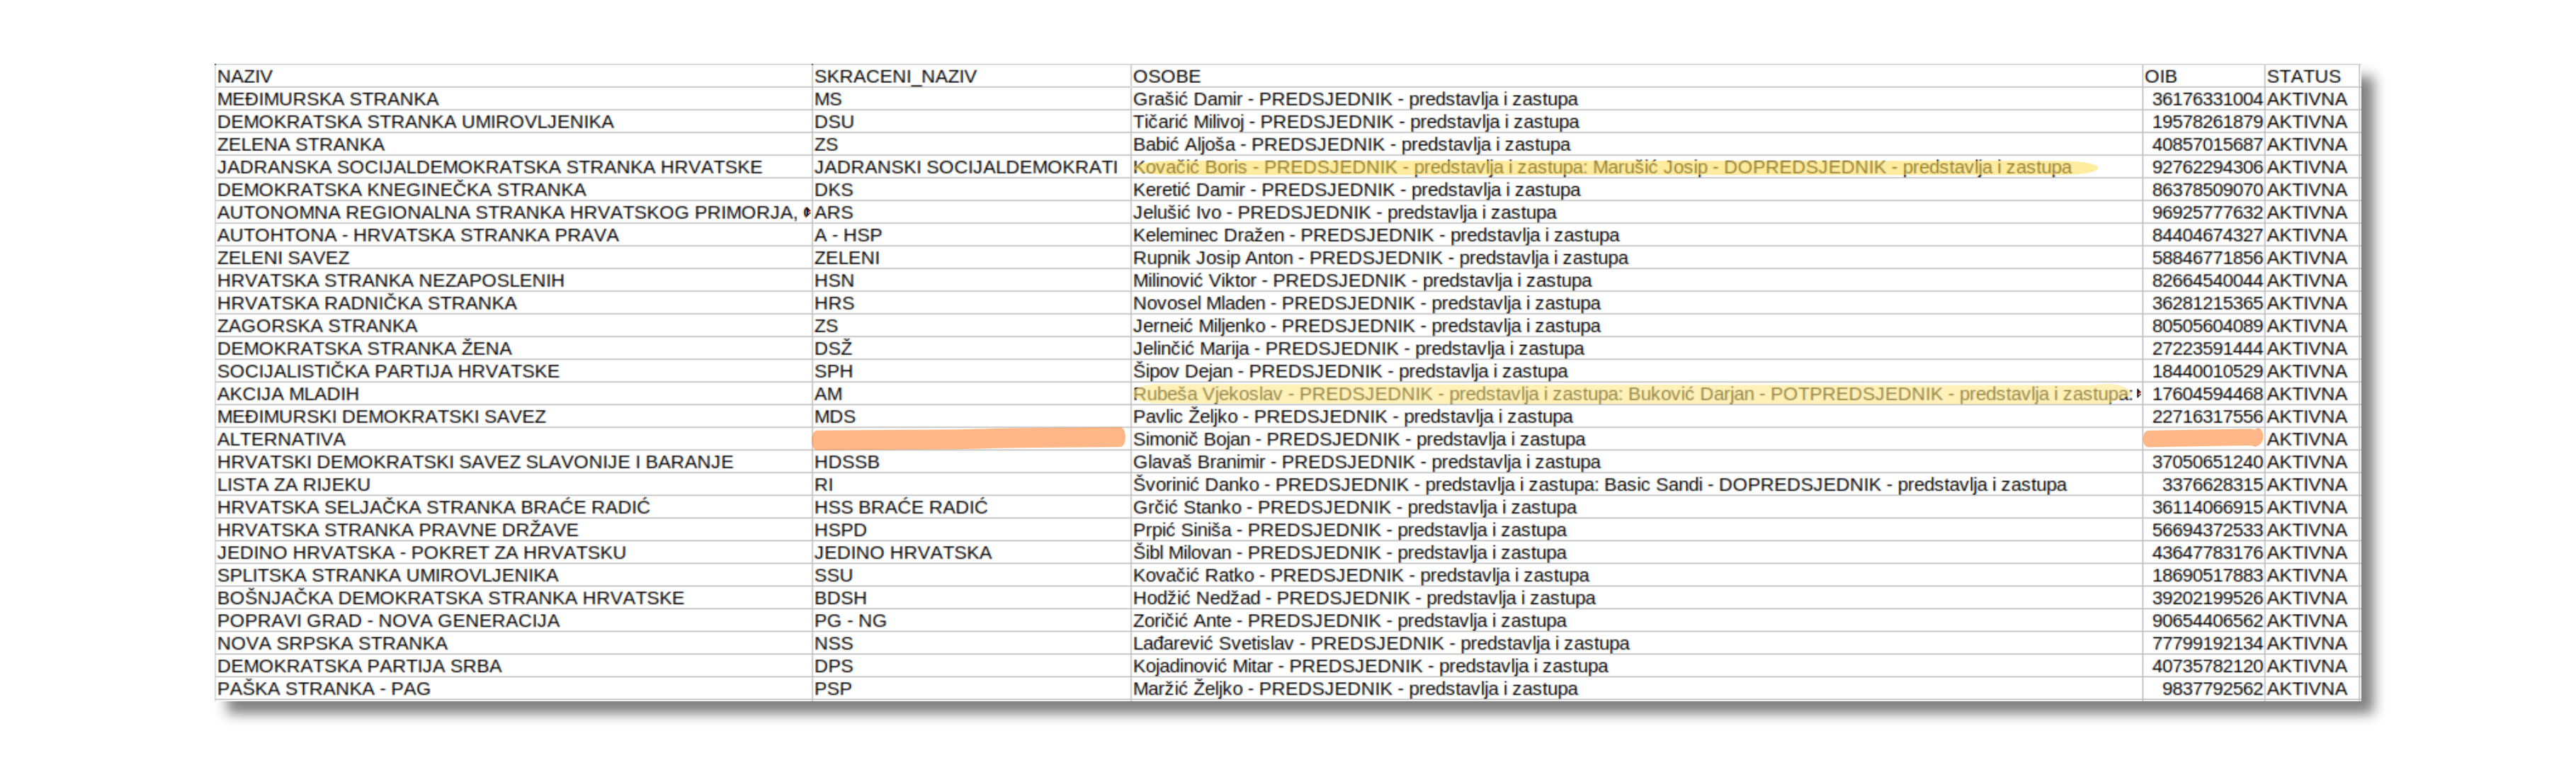
\includegraphics[scale=.27]{images/messy-politics.png}
    \end{itemize}
\end{frame}

\begin{frame}
    \begin{itemize}
        \vspace*{1em}

        \item ne koristite formatiranje ćelija za pohranu podataka

        \pause

        \vspace{1em}

        \hspace{-.8em}%
        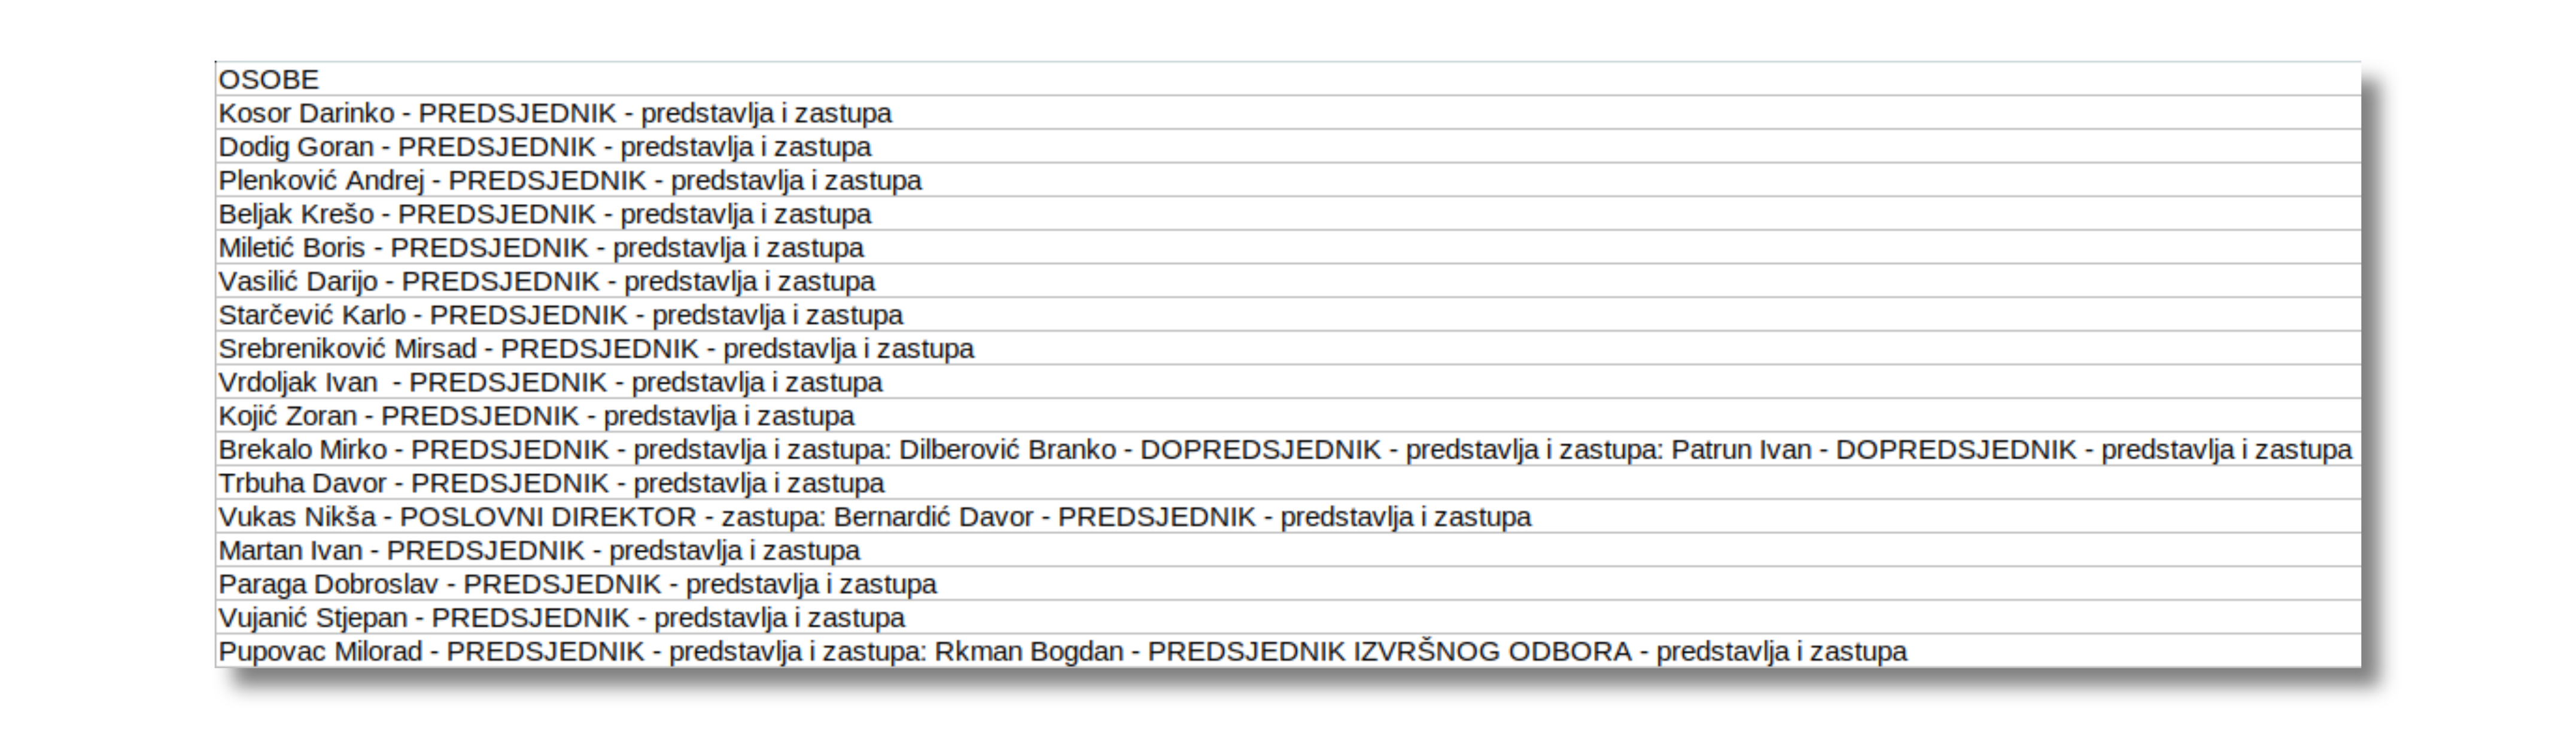
\includegraphics[scale=.30]{images/colorless-sadness.png}

        \pause
        
        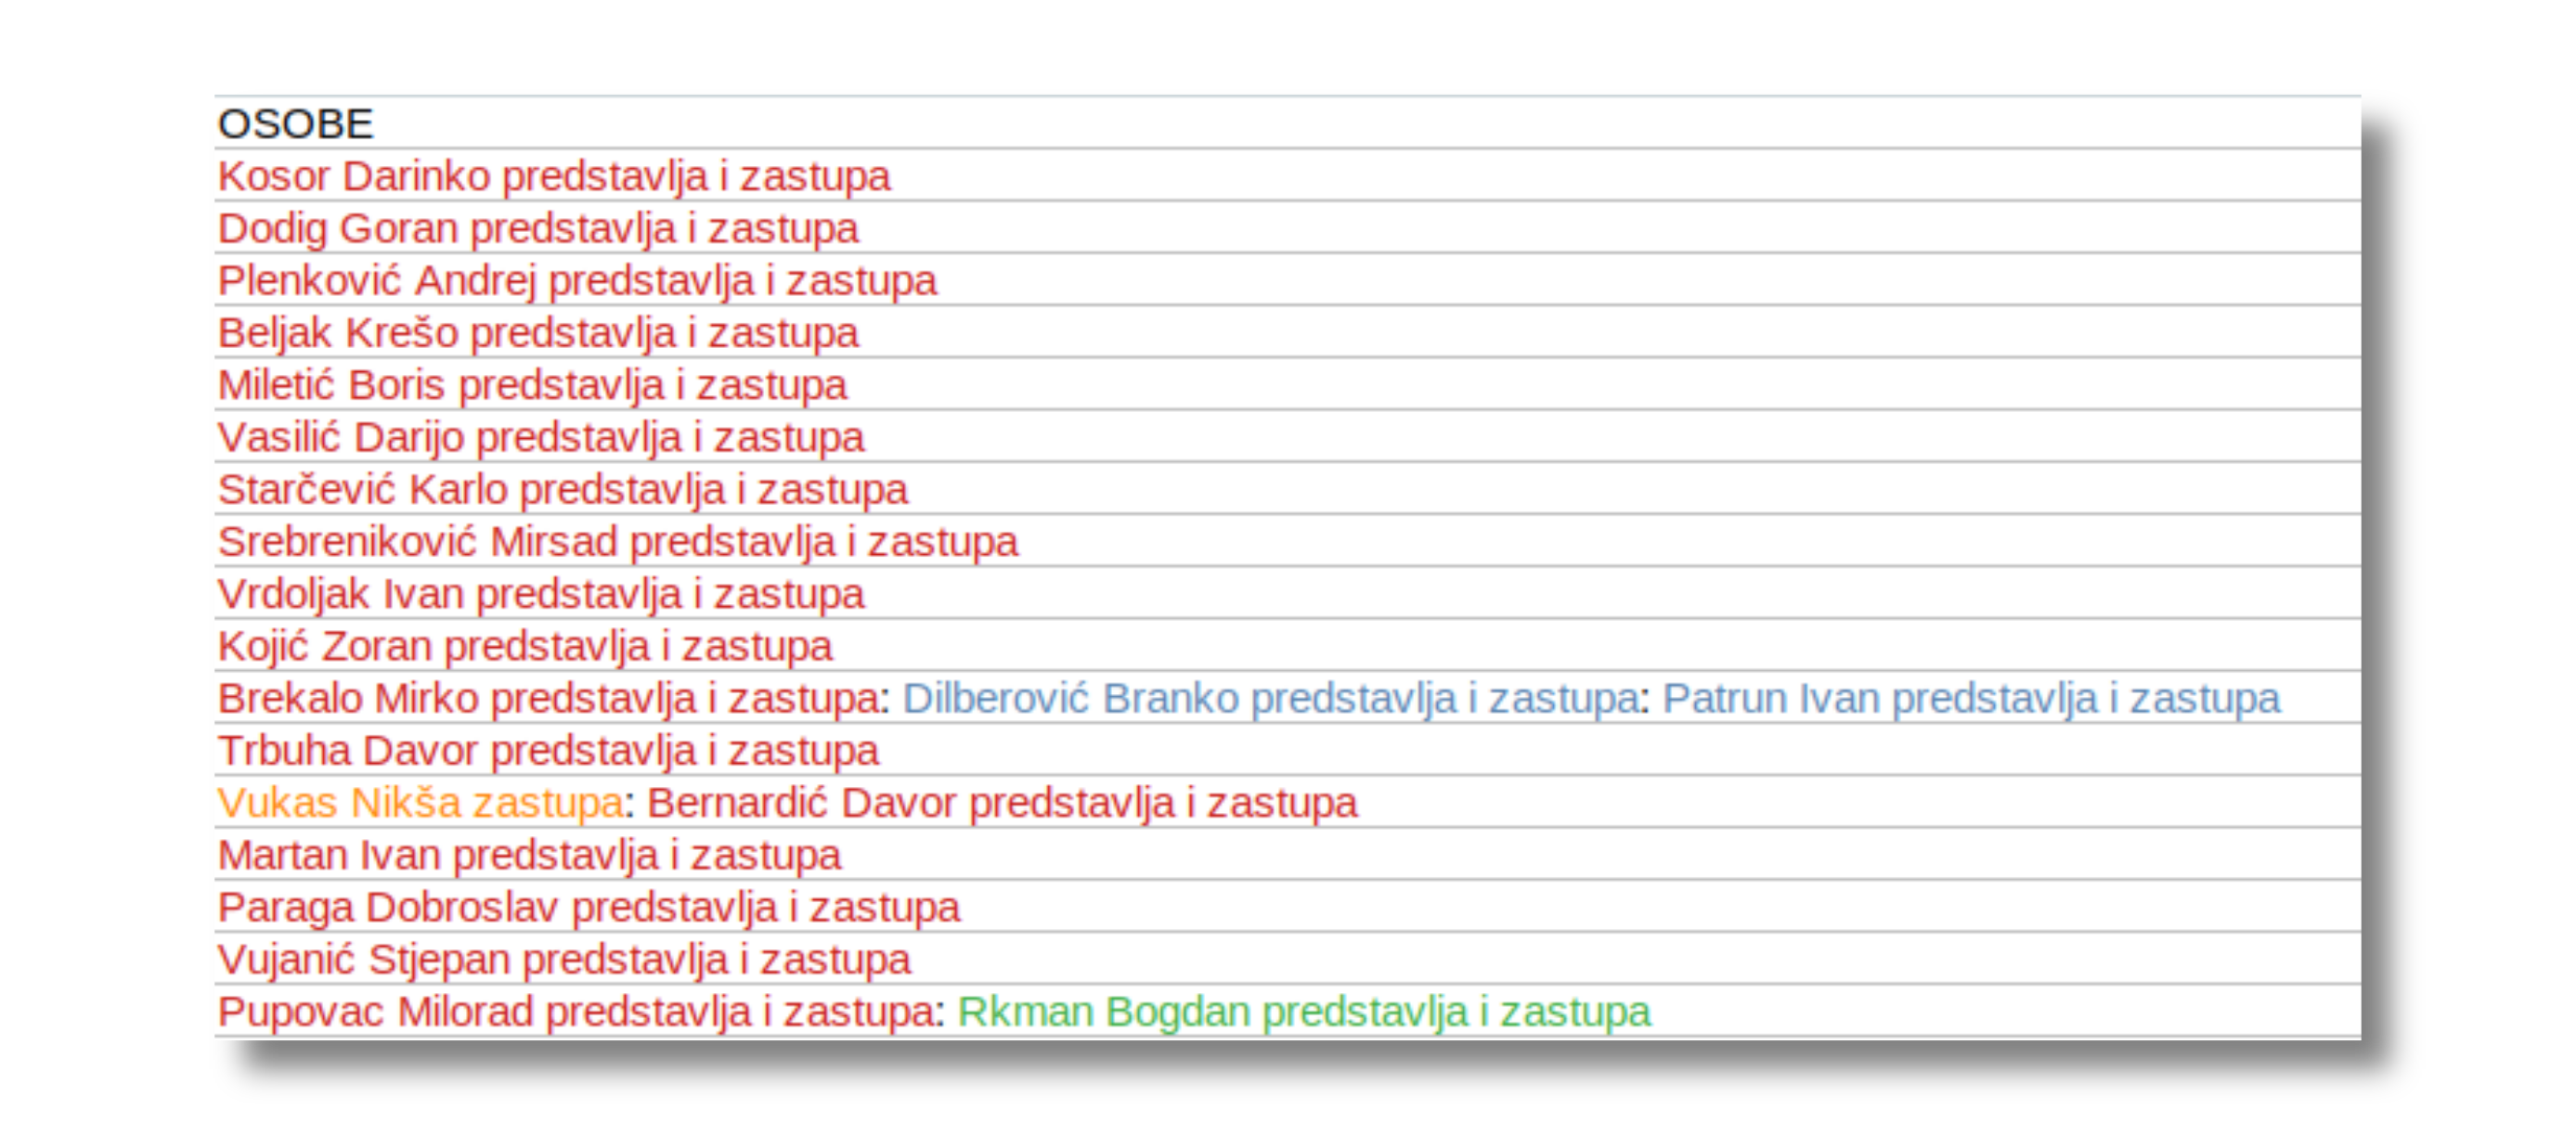
\includegraphics[scale=.30]{images/colorful-sadness.png}

    \end{itemize}
\end{frame}

\begin{frame}
    \begin{center}
        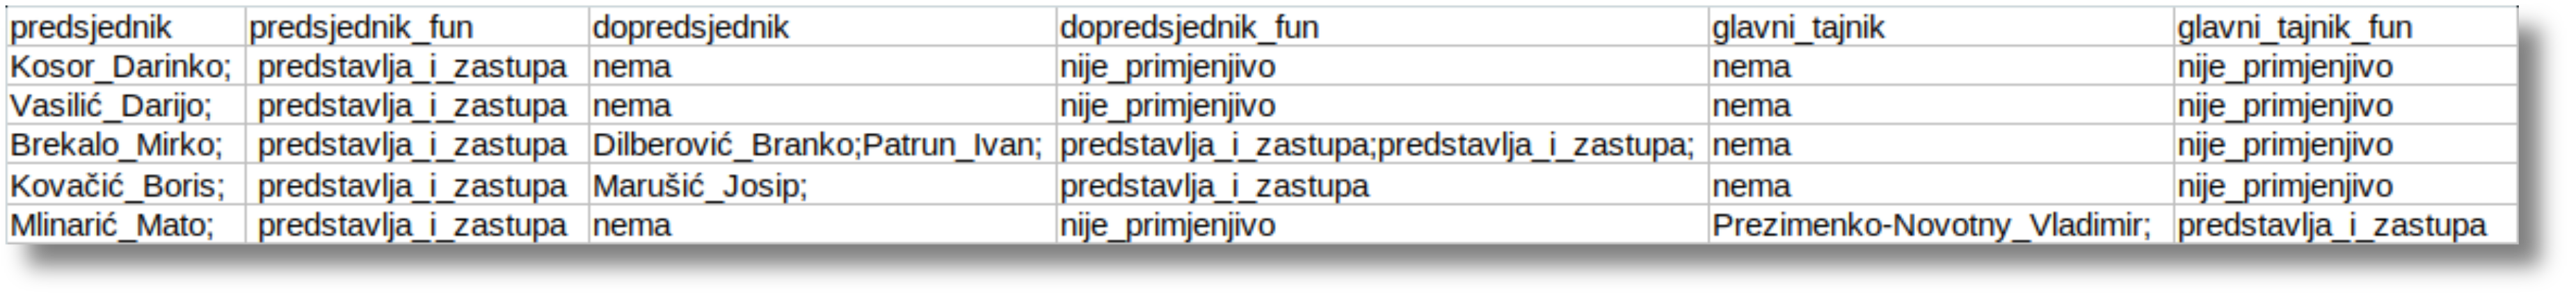
\includegraphics[scale=.45]{images/nicer-party-yes.png}
    \end{center}

    \pause

    \vspace*{3em}

    \hspace*{10em}>> There are no good ideas.\\
    \hspace{13em}-- Rory Allen Philip Ferreira
\end{frame}

\begin{frame}
    \begin{itemize}
        \setlength{\itemsep}{2em}

        \item varijablama dajte smislene nazive

            \begin{itemize}
                \item izbjegavajte posebne znakove (!, ?, @ itd.)

                \item izbjegavajte razmake (zamijenite ih s \_)

                \item izbjegavajte dijakritičke znakove (ili pazite na
                    \textit{encoding})

            \end{itemize}

            \pause

            \vspace*{1.5em}

            \begin{center}

            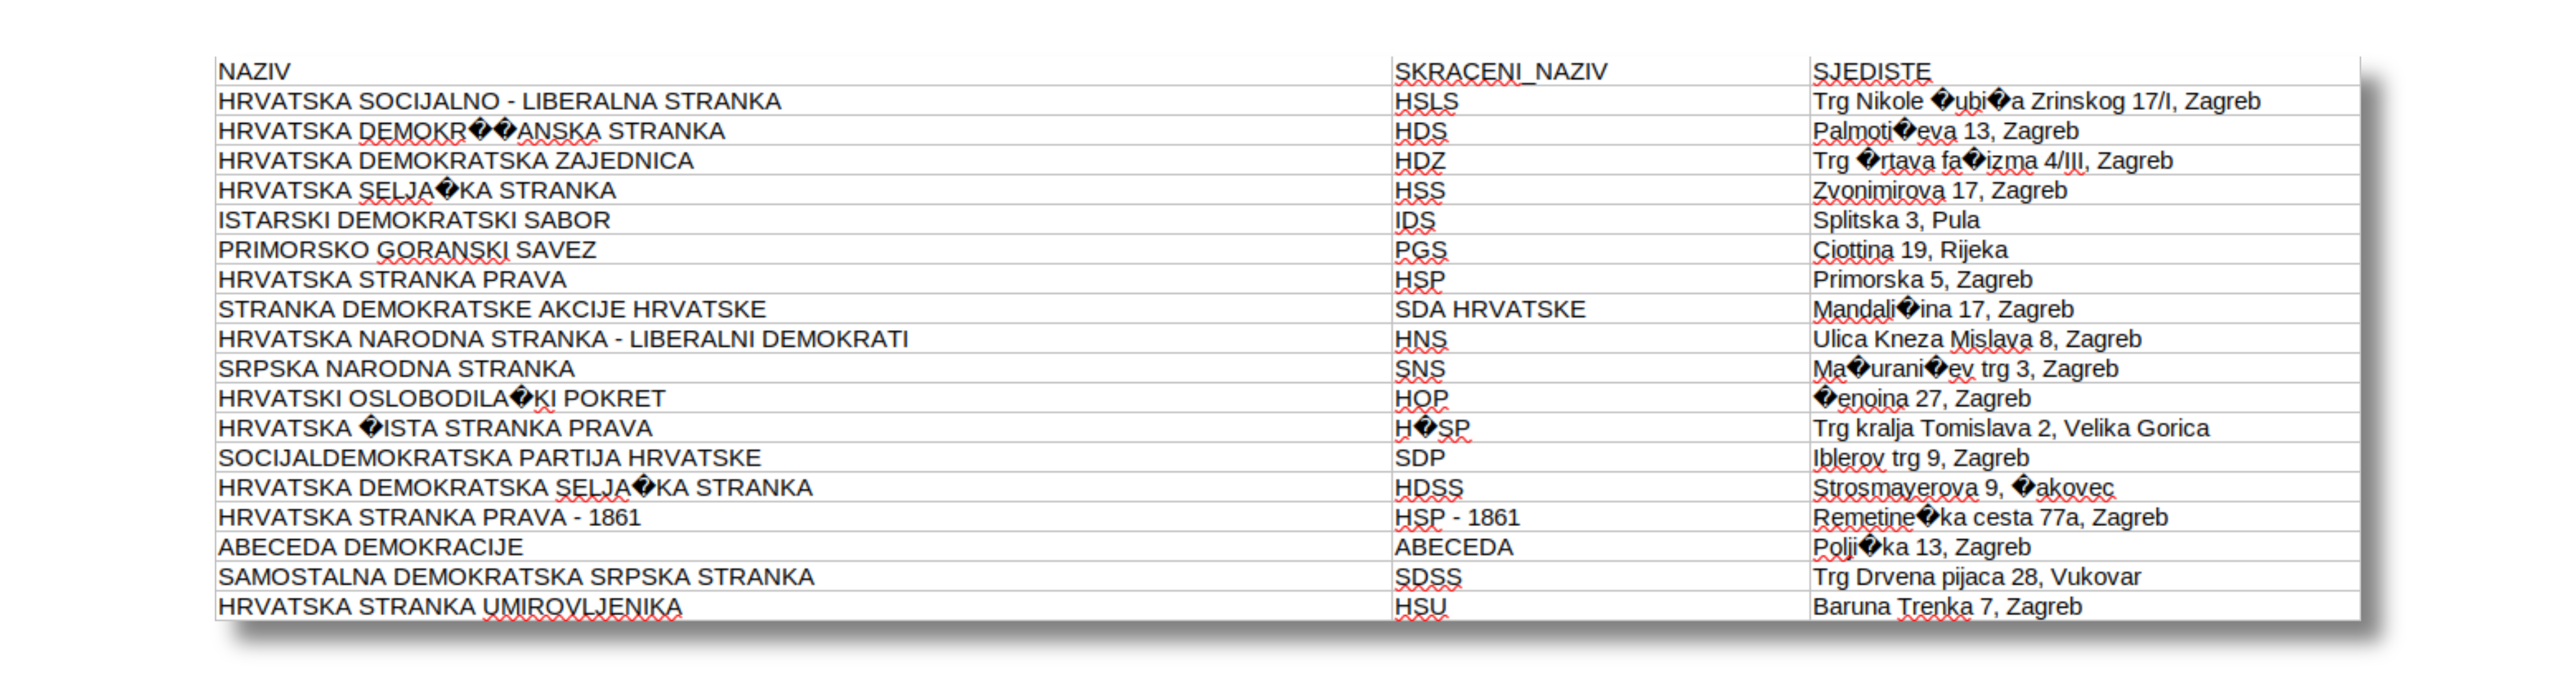
\includegraphics[scale=.32]{images/meaningless-party.png}

            \end{center}

    \end{itemize}
\end{frame}

\begin{frame}
    \begin{itemize}
        \setlength{\itemsep}{2em}

        \item \textit{nikakve} analize ili promjene u datotekama sa sirovim
            podacima

        \pause

        \item napravite sigurnosne kopije

        \pause

        \item napravite metapodatke

        \begin{itemize}
            \item ime varijable

            \item objašnjenje varijable

            \item raspon vrijednosti

        \end{itemize}

    \end{itemize}
\end{frame}

\begin{frame}
    \begin{itemize}
        \item da sve ne bude tužno

        \begin{center}
            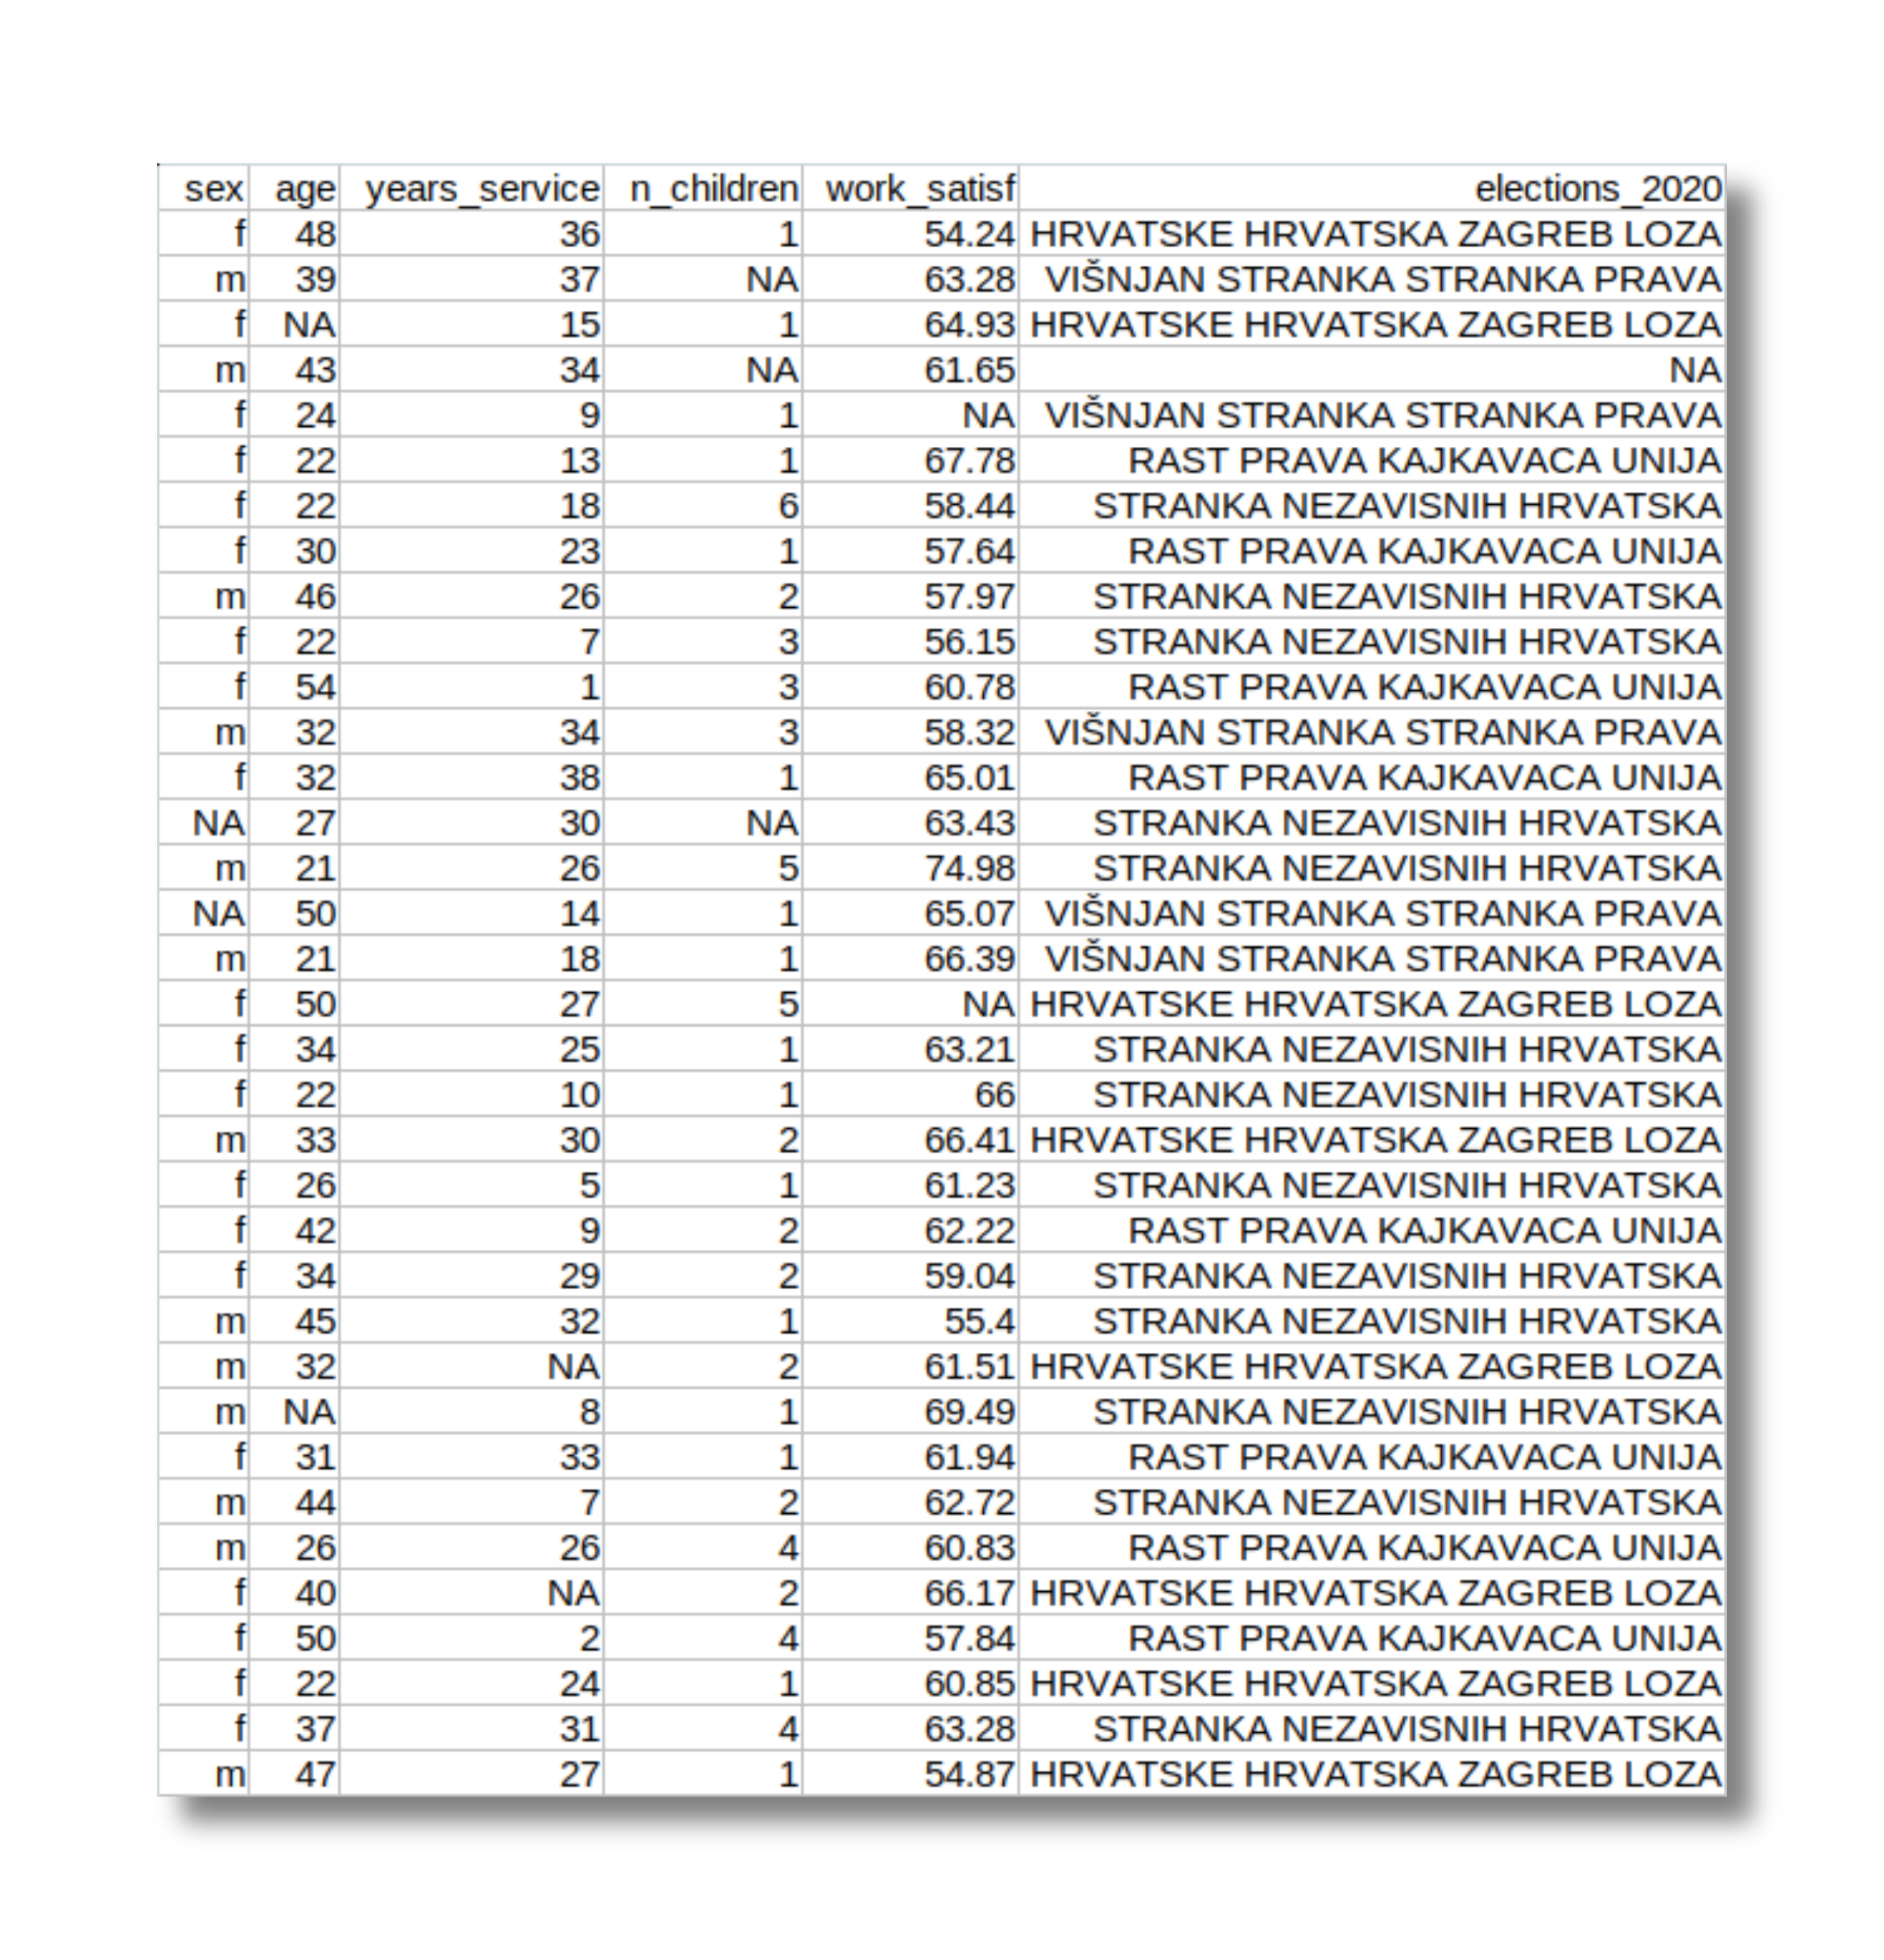
\includegraphics[scale=.30]{images/nice-but-fake.png}
        \end{center}

    \end{itemize}
\end{frame}

\begin{noheadline}
    \begin{frame}
    \fontfamily{mak}

    \fontsize{50}{52}\selectfont
    \centering
    ?
    \end{frame}
\end{noheadline}

\begin{frame}
    \frametitle{?}

    \begin{itemize}
        \setlength{\itemsep}{2em}

        \item Horor priče o podacima.

        \item Prepreke na koje ste nailazili u vlastitom radu?

    \end{itemize}

\end{frame}

\begin{noheadline}
    \begin{frame}
        \frametitle{Dodatni materijali i reference}

        \fontsize{10}{12}\selectfont

        \begin{itemize}
            \setlength{\itemsep}{1em}
            
            \item morževi preuzeti iz Kastelein, R. A., Zweypfenning, R. C. V.
                J., Spekreijse, H., Dubbeldam, J. L., i Born, E. W. (1993). The
                Anatomy of the walrus head (Odobenus rosmarus). Part 3: The eyes
                and their function in Walrus ecology. \textit{Aquatic mammals, 19},
                61-61.

            \item sadržaj temeljen na Broman, K. W., \& Woo, K. H. (2018). Data
                organization in spreadsheets. \textit{The American Statistician,
                72}(1), 2-10.
                \url{https://doi.org/10.1080/00031305.2017.1375989}

            \item dodatna inspiracija iz CESSDA Training Team (2020). \textit{CESSDA
                Data Management Expert Guide}. Bergen, Norway: CESSDA ERIC. doi:
                \url{https://doi.org/10.5281/zenodo.3820472}
            
        \end{itemize}
    \end{frame}
\end{noheadline}

\begin{noheadline}
    \begin{frame}
        \frametitle{Dodatni materijali i reference}

        \fontsize{10}{12}\selectfont

        \begin{itemize}
            \setlength{\itemsep}{1em}

            \item \textit{Why using Microsoft's tool caused Covid-19 results to
                be lost}: \url{https://www.bbc.com/news/technology-54423988}

            \item \textit{Scientists rename human genes to stop Microsoft Excel
                from misreading them as dates}:
                \url{https://www.theverge.com/2020/8/6/21355674/
                human-genes-rename-microsoft-excel-misreading-dates}
            
        \end{itemize}
    \end{frame}
\end{noheadline}
\end{document}
